% Graphic for TeX using PGF
% Title: /comptes/E105022E/univ-nantes/Algorithmique et structures de données 2/projet2/glossygloss/report/src/class_hashtable.dia
% Creator: Dia v0.97.2
% CreationDate: Fri Apr 25 17:56:42 2014
% For: E105022E
% \usepackage{tikz}
% The following commands are not supported in PSTricks at present
% We define them conditionally, so when they are implemented,
% this pgf file will use them.
\ifx\du\undefined
  \newlength{\du}
\fi
\setlength{\du}{15\unitlength}
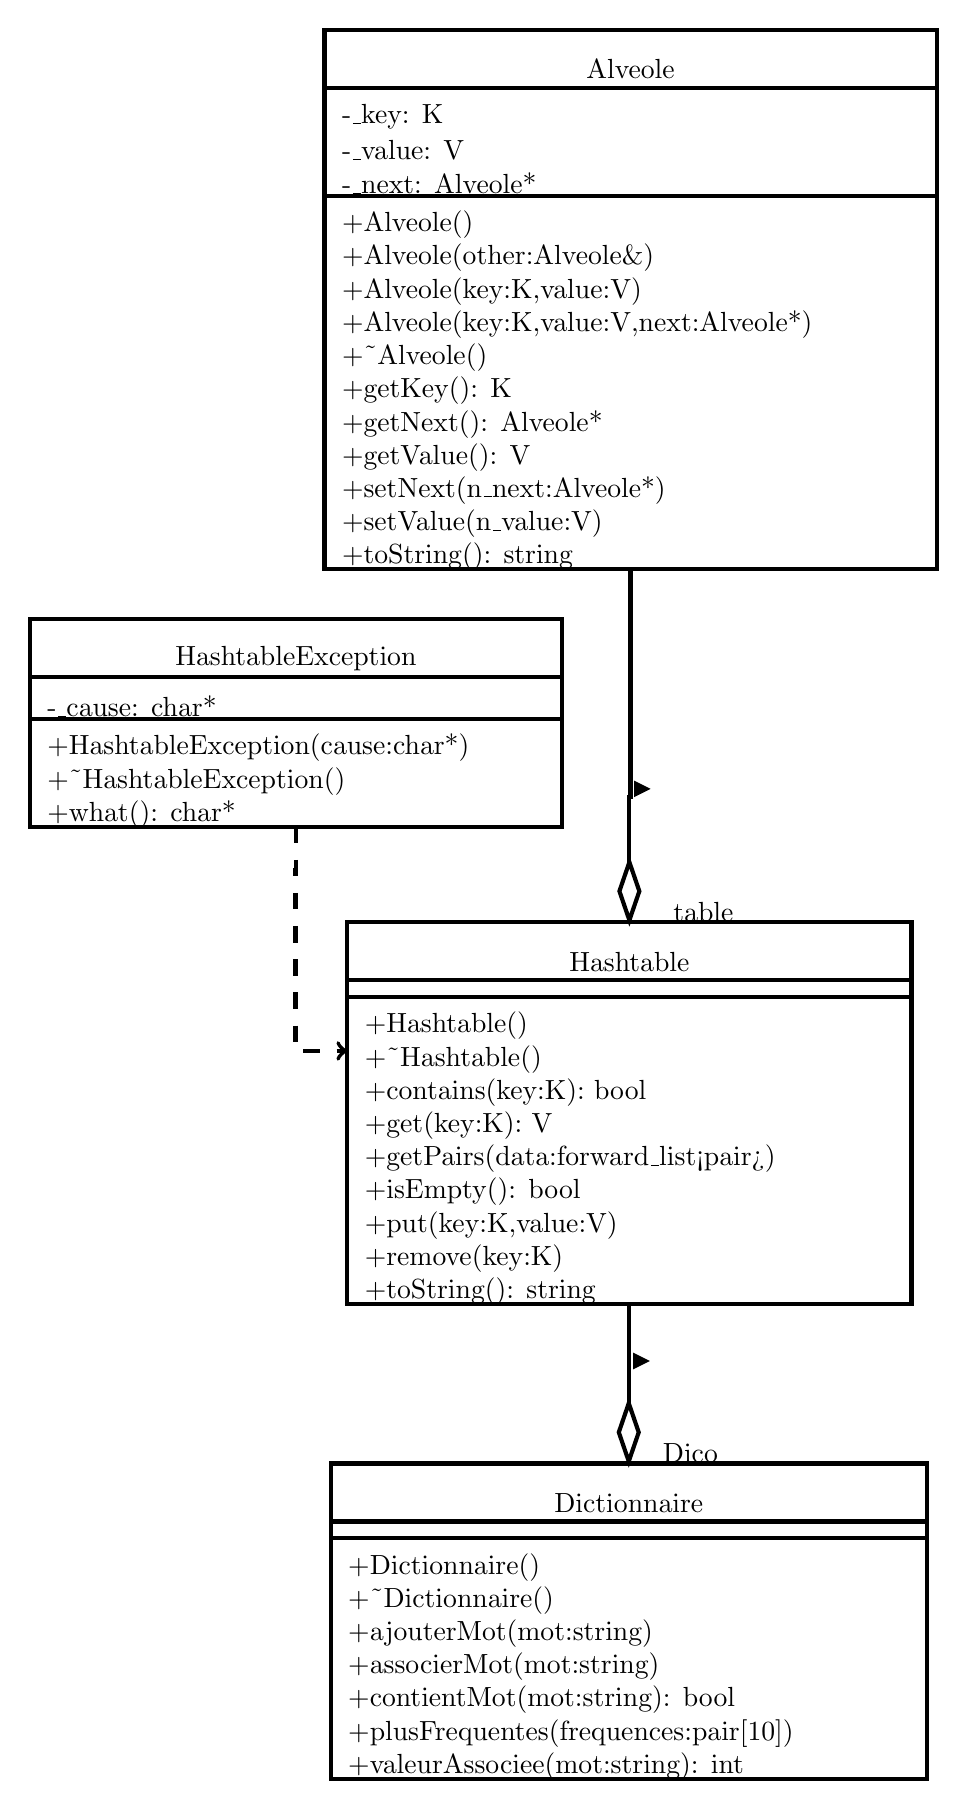
\begin{tikzpicture}
\pgftransformxscale{1.000000}
\pgftransformyscale{-1.000000}
\definecolor{dialinecolor}{rgb}{0.000000, 0.000000, 0.000000}
\pgfsetstrokecolor{dialinecolor}
\definecolor{dialinecolor}{rgb}{1.000000, 1.000000, 1.000000}
\pgfsetfillcolor{dialinecolor}
\pgfsetlinewidth{0.100000\du}
\pgfsetdash{}{0pt}
\definecolor{dialinecolor}{rgb}{1.000000, 1.000000, 1.000000}
\pgfsetfillcolor{dialinecolor}
\fill (12.450000\du,11.250000\du)--(12.450000\du,12.650000\du)--(25.270000\du,12.650000\du)--(25.270000\du,11.250000\du)--cycle;
\definecolor{dialinecolor}{rgb}{0.000000, 0.000000, 0.000000}
\pgfsetstrokecolor{dialinecolor}
\draw (12.450000\du,11.250000\du)--(12.450000\du,12.650000\du)--(25.270000\du,12.650000\du)--(25.270000\du,11.250000\du)--cycle;
% setfont left to latex
\definecolor{dialinecolor}{rgb}{0.000000, 0.000000, 0.000000}
\pgfsetstrokecolor{dialinecolor}
\node at (18.860000\du,12.200000\du){HashtableException};
\definecolor{dialinecolor}{rgb}{1.000000, 1.000000, 1.000000}
\pgfsetfillcolor{dialinecolor}
\fill (12.450000\du,12.650000\du)--(12.450000\du,13.650000\du)--(25.270000\du,13.650000\du)--(25.270000\du,12.650000\du)--cycle;
\definecolor{dialinecolor}{rgb}{0.000000, 0.000000, 0.000000}
\pgfsetstrokecolor{dialinecolor}
\draw (12.450000\du,12.650000\du)--(12.450000\du,13.650000\du)--(25.270000\du,13.650000\du)--(25.270000\du,12.650000\du)--cycle;
% setfont left to latex
\definecolor{dialinecolor}{rgb}{0.000000, 0.000000, 0.000000}
\pgfsetstrokecolor{dialinecolor}
\node[anchor=west] at (12.600000\du,13.350000\du){-\_cause: char*};
\definecolor{dialinecolor}{rgb}{1.000000, 1.000000, 1.000000}
\pgfsetfillcolor{dialinecolor}
\fill (12.450000\du,13.650000\du)--(12.450000\du,16.250000\du)--(25.270000\du,16.250000\du)--(25.270000\du,13.650000\du)--cycle;
\definecolor{dialinecolor}{rgb}{0.000000, 0.000000, 0.000000}
\pgfsetstrokecolor{dialinecolor}
\draw (12.450000\du,13.650000\du)--(12.450000\du,16.250000\du)--(25.270000\du,16.250000\du)--(25.270000\du,13.650000\du)--cycle;
% setfont left to latex
\definecolor{dialinecolor}{rgb}{0.000000, 0.000000, 0.000000}
\pgfsetstrokecolor{dialinecolor}
\node[anchor=west] at (12.600000\du,14.350000\du){+HashtableException(cause:char*)};
% setfont left to latex
\definecolor{dialinecolor}{rgb}{0.000000, 0.000000, 0.000000}
\pgfsetstrokecolor{dialinecolor}
\node[anchor=west] at (12.600000\du,15.150000\du){+\~{}HashtableException()};
% setfont left to latex
\definecolor{dialinecolor}{rgb}{0.000000, 0.000000, 0.000000}
\pgfsetstrokecolor{dialinecolor}
\node[anchor=west] at (12.600000\du,15.950000\du){+what(): char*};
\pgfsetlinewidth{0.100000\du}
\pgfsetdash{}{0pt}
\definecolor{dialinecolor}{rgb}{1.000000, 1.000000, 1.000000}
\pgfsetfillcolor{dialinecolor}
\fill (19.550000\du,-2.950000\du)--(19.550000\du,-1.550000\du)--(34.295000\du,-1.550000\du)--(34.295000\du,-2.950000\du)--cycle;
\definecolor{dialinecolor}{rgb}{0.000000, 0.000000, 0.000000}
\pgfsetstrokecolor{dialinecolor}
\draw (19.550000\du,-2.950000\du)--(19.550000\du,-1.550000\du)--(34.295000\du,-1.550000\du)--(34.295000\du,-2.950000\du)--cycle;
% setfont left to latex
\definecolor{dialinecolor}{rgb}{0.000000, 0.000000, 0.000000}
\pgfsetstrokecolor{dialinecolor}
\node at (26.922500\du,-2.000000\du){Alveole};
\definecolor{dialinecolor}{rgb}{1.000000, 1.000000, 1.000000}
\pgfsetfillcolor{dialinecolor}
\fill (19.550000\du,-1.550000\du)--(19.550000\du,1.050000\du)--(34.295000\du,1.050000\du)--(34.295000\du,-1.550000\du)--cycle;
\definecolor{dialinecolor}{rgb}{0.000000, 0.000000, 0.000000}
\pgfsetstrokecolor{dialinecolor}
\draw (19.550000\du,-1.550000\du)--(19.550000\du,1.050000\du)--(34.295000\du,1.050000\du)--(34.295000\du,-1.550000\du)--cycle;
% setfont left to latex
\definecolor{dialinecolor}{rgb}{0.000000, 0.000000, 0.000000}
\pgfsetstrokecolor{dialinecolor}
\node[anchor=west] at (19.700000\du,-0.850000\du){-\_key: K};
% setfont left to latex
\definecolor{dialinecolor}{rgb}{0.000000, 0.000000, 0.000000}
\pgfsetstrokecolor{dialinecolor}
\node[anchor=west] at (19.700000\du,-0.050000\du){-\_value: V};
% setfont left to latex
\definecolor{dialinecolor}{rgb}{0.000000, 0.000000, 0.000000}
\pgfsetstrokecolor{dialinecolor}
\node[anchor=west] at (19.700000\du,0.750000\du){-\_next: Alveole*};
\definecolor{dialinecolor}{rgb}{1.000000, 1.000000, 1.000000}
\pgfsetfillcolor{dialinecolor}
\fill (19.550000\du,1.050000\du)--(19.550000\du,10.050000\du)--(34.295000\du,10.050000\du)--(34.295000\du,1.050000\du)--cycle;
\definecolor{dialinecolor}{rgb}{0.000000, 0.000000, 0.000000}
\pgfsetstrokecolor{dialinecolor}
\draw (19.550000\du,1.050000\du)--(19.550000\du,10.050000\du)--(34.295000\du,10.050000\du)--(34.295000\du,1.050000\du)--cycle;
% setfont left to latex
\definecolor{dialinecolor}{rgb}{0.000000, 0.000000, 0.000000}
\pgfsetstrokecolor{dialinecolor}
\node[anchor=west] at (19.700000\du,1.750000\du){+Alveole()};
% setfont left to latex
\definecolor{dialinecolor}{rgb}{0.000000, 0.000000, 0.000000}
\pgfsetstrokecolor{dialinecolor}
\node[anchor=west] at (19.700000\du,2.550000\du){+Alveole(other:Alveole\&)};
% setfont left to latex
\definecolor{dialinecolor}{rgb}{0.000000, 0.000000, 0.000000}
\pgfsetstrokecolor{dialinecolor}
\node[anchor=west] at (19.700000\du,3.350000\du){+Alveole(key:K,value:V)};
% setfont left to latex
\definecolor{dialinecolor}{rgb}{0.000000, 0.000000, 0.000000}
\pgfsetstrokecolor{dialinecolor}
\node[anchor=west] at (19.700000\du,4.150000\du){+Alveole(key:K,value:V,next:Alveole*)};
% setfont left to latex
\definecolor{dialinecolor}{rgb}{0.000000, 0.000000, 0.000000}
\pgfsetstrokecolor{dialinecolor}
\node[anchor=west] at (19.700000\du,4.950000\du){+\~{}Alveole()};
% setfont left to latex
\definecolor{dialinecolor}{rgb}{0.000000, 0.000000, 0.000000}
\pgfsetstrokecolor{dialinecolor}
\node[anchor=west] at (19.700000\du,5.750000\du){+getKey(): K};
% setfont left to latex
\definecolor{dialinecolor}{rgb}{0.000000, 0.000000, 0.000000}
\pgfsetstrokecolor{dialinecolor}
\node[anchor=west] at (19.700000\du,6.550000\du){+getNext(): Alveole*};
% setfont left to latex
\definecolor{dialinecolor}{rgb}{0.000000, 0.000000, 0.000000}
\pgfsetstrokecolor{dialinecolor}
\node[anchor=west] at (19.700000\du,7.350000\du){+getValue(): V};
% setfont left to latex
\definecolor{dialinecolor}{rgb}{0.000000, 0.000000, 0.000000}
\pgfsetstrokecolor{dialinecolor}
\node[anchor=west] at (19.700000\du,8.150000\du){+setNext(n\_next:Alveole*)};
% setfont left to latex
\definecolor{dialinecolor}{rgb}{0.000000, 0.000000, 0.000000}
\pgfsetstrokecolor{dialinecolor}
\node[anchor=west] at (19.700000\du,8.950000\du){+setValue(n\_value:V)};
% setfont left to latex
\definecolor{dialinecolor}{rgb}{0.000000, 0.000000, 0.000000}
\pgfsetstrokecolor{dialinecolor}
\node[anchor=west] at (19.700000\du,9.750000\du){+toString(): string};
\pgfsetlinewidth{0.100000\du}
\pgfsetdash{}{0pt}
\definecolor{dialinecolor}{rgb}{1.000000, 1.000000, 1.000000}
\pgfsetfillcolor{dialinecolor}
\fill (20.100000\du,18.550000\du)--(20.100000\du,19.950000\du)--(33.690000\du,19.950000\du)--(33.690000\du,18.550000\du)--cycle;
\definecolor{dialinecolor}{rgb}{0.000000, 0.000000, 0.000000}
\pgfsetstrokecolor{dialinecolor}
\draw (20.100000\du,18.550000\du)--(20.100000\du,19.950000\du)--(33.690000\du,19.950000\du)--(33.690000\du,18.550000\du)--cycle;
% setfont left to latex
\definecolor{dialinecolor}{rgb}{0.000000, 0.000000, 0.000000}
\pgfsetstrokecolor{dialinecolor}
\node at (26.895000\du,19.500000\du){Hashtable};
\definecolor{dialinecolor}{rgb}{1.000000, 1.000000, 1.000000}
\pgfsetfillcolor{dialinecolor}
\fill (20.100000\du,19.950000\du)--(20.100000\du,20.350000\du)--(33.690000\du,20.350000\du)--(33.690000\du,19.950000\du)--cycle;
\definecolor{dialinecolor}{rgb}{0.000000, 0.000000, 0.000000}
\pgfsetstrokecolor{dialinecolor}
\draw (20.100000\du,19.950000\du)--(20.100000\du,20.350000\du)--(33.690000\du,20.350000\du)--(33.690000\du,19.950000\du)--cycle;
\definecolor{dialinecolor}{rgb}{1.000000, 1.000000, 1.000000}
\pgfsetfillcolor{dialinecolor}
\fill (20.100000\du,20.350000\du)--(20.100000\du,27.750000\du)--(33.690000\du,27.750000\du)--(33.690000\du,20.350000\du)--cycle;
\definecolor{dialinecolor}{rgb}{0.000000, 0.000000, 0.000000}
\pgfsetstrokecolor{dialinecolor}
\draw (20.100000\du,20.350000\du)--(20.100000\du,27.750000\du)--(33.690000\du,27.750000\du)--(33.690000\du,20.350000\du)--cycle;
% setfont left to latex
\definecolor{dialinecolor}{rgb}{0.000000, 0.000000, 0.000000}
\pgfsetstrokecolor{dialinecolor}
\node[anchor=west] at (20.250000\du,21.050000\du){+Hashtable()};
% setfont left to latex
\definecolor{dialinecolor}{rgb}{0.000000, 0.000000, 0.000000}
\pgfsetstrokecolor{dialinecolor}
\node[anchor=west] at (20.250000\du,21.850000\du){+\~{}Hashtable()};
% setfont left to latex
\definecolor{dialinecolor}{rgb}{0.000000, 0.000000, 0.000000}
\pgfsetstrokecolor{dialinecolor}
\node[anchor=west] at (20.250000\du,22.650000\du){+contains(key:K): bool};
% setfont left to latex
\definecolor{dialinecolor}{rgb}{0.000000, 0.000000, 0.000000}
\pgfsetstrokecolor{dialinecolor}
\node[anchor=west] at (20.250000\du,23.450000\du){+get(key:K): V};
% setfont left to latex
\definecolor{dialinecolor}{rgb}{0.000000, 0.000000, 0.000000}
\pgfsetstrokecolor{dialinecolor}
\node[anchor=west] at (20.250000\du,24.250000\du){+getPairs(data:forward\_list<pair>)};
% setfont left to latex
\definecolor{dialinecolor}{rgb}{0.000000, 0.000000, 0.000000}
\pgfsetstrokecolor{dialinecolor}
\node[anchor=west] at (20.250000\du,25.050000\du){+isEmpty(): bool};
% setfont left to latex
\definecolor{dialinecolor}{rgb}{0.000000, 0.000000, 0.000000}
\pgfsetstrokecolor{dialinecolor}
\node[anchor=west] at (20.250000\du,25.850000\du){+put(key:K,value:V)};
% setfont left to latex
\definecolor{dialinecolor}{rgb}{0.000000, 0.000000, 0.000000}
\pgfsetstrokecolor{dialinecolor}
\node[anchor=west] at (20.250000\du,26.650000\du){+remove(key:K)};
% setfont left to latex
\definecolor{dialinecolor}{rgb}{0.000000, 0.000000, 0.000000}
\pgfsetstrokecolor{dialinecolor}
\node[anchor=west] at (20.250000\du,27.450000\du){+toString(): string};
\pgfsetlinewidth{0.100000\du}
\pgfsetdash{{1.000000\du}{1.000000\du}}{0\du}
\pgfsetdash{{0.400000\du}{0.400000\du}}{0\du}
\pgfsetmiterjoin
\pgfsetbuttcap
{
\definecolor{dialinecolor}{rgb}{0.000000, 0.000000, 0.000000}
\pgfsetfillcolor{dialinecolor}
% was here!!!
\pgfsetarrowsend{to}
\definecolor{dialinecolor}{rgb}{0.000000, 0.000000, 0.000000}
\pgfsetstrokecolor{dialinecolor}
\draw (18.860000\du,16.250000\du)--(18.860000\du,17.300000\du)--(18.850000\du,17.300000\du)--(18.850000\du,21.650000\du)--(20.100000\du,21.650000\du);
}
% setfont left to latex
\pgfsetlinewidth{0.100000\du}
\pgfsetdash{}{0pt}
\pgfsetmiterjoin
\pgfsetbuttcap
{
\definecolor{dialinecolor}{rgb}{0.000000, 0.000000, 0.000000}
\pgfsetfillcolor{dialinecolor}
% was here!!!
\definecolor{dialinecolor}{rgb}{0.000000, 0.000000, 0.000000}
\pgfsetstrokecolor{dialinecolor}
\draw (26.895000\du,18.501840\du)--(26.895000\du,15.537500\du)--(26.922500\du,15.537500\du)--(26.922500\du,10.050000\du);
}
\definecolor{dialinecolor}{rgb}{0.000000, 0.000000, 0.000000}
\pgfsetstrokecolor{dialinecolor}
\draw (26.895000\du,17.243262\du)--(26.895000\du,15.537500\du)--(26.922500\du,15.537500\du)--(26.922500\du,10.050000\du);
\pgfsetdash{}{0pt}
\pgfsetmiterjoin
\pgfsetbuttcap
\definecolor{dialinecolor}{rgb}{1.000000, 1.000000, 1.000000}
\pgfsetfillcolor{dialinecolor}
\fill (26.895000\du,18.501840\du)--(26.655000\du,17.801840\du)--(26.895000\du,17.101840\du)--(27.135000\du,17.801840\du)--cycle;
\pgfsetlinewidth{0.100000\du}
\pgfsetdash{}{0pt}
\pgfsetmiterjoin
\pgfsetbuttcap
\definecolor{dialinecolor}{rgb}{0.000000, 0.000000, 0.000000}
\pgfsetstrokecolor{dialinecolor}
\draw (26.895000\du,18.501840\du)--(26.655000\du,17.801840\du)--(26.895000\du,17.101840\du)--(27.135000\du,17.801840\du)--cycle;
% setfont left to latex
\definecolor{dialinecolor}{rgb}{0.000000, 0.000000, 0.000000}
\pgfsetfillcolor{dialinecolor}
\fill (27.008750\du,15.537500\du)--(27.008750\du,15.137500\du)--(27.408750\du,15.337500\du)--cycle;
\definecolor{dialinecolor}{rgb}{0.000000, 0.000000, 0.000000}
\pgfsetstrokecolor{dialinecolor}
\node[anchor=west] at (27.445000\du,18.301840\du){ \_table};
\pgfsetlinewidth{0.100000\du}
\pgfsetdash{}{0pt}
\definecolor{dialinecolor}{rgb}{1.000000, 1.000000, 1.000000}
\pgfsetfillcolor{dialinecolor}
\fill (19.700000\du,31.587500\du)--(19.700000\du,32.987500\du)--(34.060000\du,32.987500\du)--(34.060000\du,31.587500\du)--cycle;
\definecolor{dialinecolor}{rgb}{0.000000, 0.000000, 0.000000}
\pgfsetstrokecolor{dialinecolor}
\draw (19.700000\du,31.587500\du)--(19.700000\du,32.987500\du)--(34.060000\du,32.987500\du)--(34.060000\du,31.587500\du)--cycle;
% setfont left to latex
\definecolor{dialinecolor}{rgb}{0.000000, 0.000000, 0.000000}
\pgfsetstrokecolor{dialinecolor}
\node at (26.880000\du,32.537500\du){Dictionnaire};
\definecolor{dialinecolor}{rgb}{1.000000, 1.000000, 1.000000}
\pgfsetfillcolor{dialinecolor}
\fill (19.700000\du,32.987500\du)--(19.700000\du,33.387500\du)--(34.060000\du,33.387500\du)--(34.060000\du,32.987500\du)--cycle;
\definecolor{dialinecolor}{rgb}{0.000000, 0.000000, 0.000000}
\pgfsetstrokecolor{dialinecolor}
\draw (19.700000\du,32.987500\du)--(19.700000\du,33.387500\du)--(34.060000\du,33.387500\du)--(34.060000\du,32.987500\du)--cycle;
\definecolor{dialinecolor}{rgb}{1.000000, 1.000000, 1.000000}
\pgfsetfillcolor{dialinecolor}
\fill (19.700000\du,33.387500\du)--(19.700000\du,39.187500\du)--(34.060000\du,39.187500\du)--(34.060000\du,33.387500\du)--cycle;
\definecolor{dialinecolor}{rgb}{0.000000, 0.000000, 0.000000}
\pgfsetstrokecolor{dialinecolor}
\draw (19.700000\du,33.387500\du)--(19.700000\du,39.187500\du)--(34.060000\du,39.187500\du)--(34.060000\du,33.387500\du)--cycle;
% setfont left to latex
\definecolor{dialinecolor}{rgb}{0.000000, 0.000000, 0.000000}
\pgfsetstrokecolor{dialinecolor}
\node[anchor=west] at (19.850000\du,34.087500\du){+Dictionnaire()};
% setfont left to latex
\definecolor{dialinecolor}{rgb}{0.000000, 0.000000, 0.000000}
\pgfsetstrokecolor{dialinecolor}
\node[anchor=west] at (19.850000\du,34.887500\du){+\~{}Dictionnaire()};
% setfont left to latex
\definecolor{dialinecolor}{rgb}{0.000000, 0.000000, 0.000000}
\pgfsetstrokecolor{dialinecolor}
\node[anchor=west] at (19.850000\du,35.687500\du){+ajouterMot(mot:string)};
% setfont left to latex
\definecolor{dialinecolor}{rgb}{0.000000, 0.000000, 0.000000}
\pgfsetstrokecolor{dialinecolor}
\node[anchor=west] at (19.850000\du,36.487500\du){+associerMot(mot:string)};
% setfont left to latex
\definecolor{dialinecolor}{rgb}{0.000000, 0.000000, 0.000000}
\pgfsetstrokecolor{dialinecolor}
\node[anchor=west] at (19.850000\du,37.287500\du){+contientMot(mot:string): bool};
% setfont left to latex
\definecolor{dialinecolor}{rgb}{0.000000, 0.000000, 0.000000}
\pgfsetstrokecolor{dialinecolor}
\node[anchor=west] at (19.850000\du,38.087500\du){+plusFrequentes(frequences:pair\ensuremath{[}10\ensuremath{]})};
% setfont left to latex
\definecolor{dialinecolor}{rgb}{0.000000, 0.000000, 0.000000}
\pgfsetstrokecolor{dialinecolor}
\node[anchor=west] at (19.850000\du,38.887500\du){+valeurAssociee(mot:string): int};
\pgfsetlinewidth{0.100000\du}
\pgfsetdash{}{0pt}
\pgfsetmiterjoin
\pgfsetbuttcap
{
\definecolor{dialinecolor}{rgb}{0.000000, 0.000000, 0.000000}
\pgfsetfillcolor{dialinecolor}
% was here!!!
\definecolor{dialinecolor}{rgb}{0.000000, 0.000000, 0.000000}
\pgfsetstrokecolor{dialinecolor}
\draw (26.880000\du,31.537030\du)--(26.880000\du,29.318657\du)--(26.895000\du,29.318657\du)--(26.895000\du,27.800284\du);
}
\definecolor{dialinecolor}{rgb}{0.000000, 0.000000, 0.000000}
\pgfsetstrokecolor{dialinecolor}
\draw (26.880000\du,30.278451\du)--(26.880000\du,29.318657\du)--(26.895000\du,29.318657\du)--(26.895000\du,27.800284\du);
\pgfsetdash{}{0pt}
\pgfsetmiterjoin
\pgfsetbuttcap
\definecolor{dialinecolor}{rgb}{1.000000, 1.000000, 1.000000}
\pgfsetfillcolor{dialinecolor}
\fill (26.880000\du,31.537030\du)--(26.640000\du,30.837030\du)--(26.880000\du,30.137030\du)--(27.120000\du,30.837030\du)--cycle;
\pgfsetlinewidth{0.100000\du}
\pgfsetdash{}{0pt}
\pgfsetmiterjoin
\pgfsetbuttcap
\definecolor{dialinecolor}{rgb}{0.000000, 0.000000, 0.000000}
\pgfsetstrokecolor{dialinecolor}
\draw (26.880000\du,31.537030\du)--(26.640000\du,30.837030\du)--(26.880000\du,30.137030\du)--(27.120000\du,30.837030\du)--cycle;
% setfont left to latex
\definecolor{dialinecolor}{rgb}{0.000000, 0.000000, 0.000000}
\pgfsetfillcolor{dialinecolor}
\fill (26.987500\du,29.318657\du)--(26.987500\du,28.918657\du)--(27.387500\du,29.118657\du)--cycle;
\definecolor{dialinecolor}{rgb}{0.000000, 0.000000, 0.000000}
\pgfsetstrokecolor{dialinecolor}
\node[anchor=west] at (27.430000\du,31.337030\du){ Dico};
\end{tikzpicture}
